\documentclass[12pt,a4paper]{article}
\usepackage[utf8]{inputenc}
\usepackage[T2A]{fontenc}
\usepackage[russian]{babel}
\usepackage{amsmath}
\usepackage{amsfonts}
\usepackage{amssymb}
\usepackage{graphicx}
\usepackage{geometry}
\usepackage{indentfirst}
\usepackage{array}
\usepackage{float}
\usepackage{booktabs}
\usepackage{caption}

\geometry{left=2.5cm, right=1.5cm, top=2cm, bottom=2cm}

\begin{document}

\begin{titlepage}
    \begin{center}
        \textbf{МОСКОВСКИЙ ФИЗИКО-ТЕХНИЧЕСКИЙ ИНСТИТУТ} \\
        \textbf{(НАЦИОНАЛЬНЫЙ ИССЛЕДОВАТЕЛЬСКИЙ УНИВЕРСИТЕТ)}
        \\[1cm]
        {\large Физтех-школа аэрокосмических технологий}
        \\[3.5cm]
        {\Huge \textbf{Атмосферно-вакуумная сверхзвуковая аэродинамическая труба}}
        \\[0.5cm]
        {\large Лабораторная работа №\,14 (СТ-4)}
        \\[1.5cm]
        \begin{flushright}
            \begin{tabular}{l l}
                Ларькин Глеб & Б03-301 \\ 
                Мурашев Артём & Б03-305 \\
                Хабибуллин Марат & Б03-305 \\
                Скворцов Максим & Б03-305 \\
            \end{tabular}
        \end{flushright}
        \vfill
        {\large Долгопрудный, 2026 г.}
    \end{center}
\end{titlepage}

\tableofcontents
\newpage

% ---------------------------------------------------------------
\section{Цель работы}
% ---------------------------------------------------------------
Цель лабораторной работы - ознакомление с работой атмосферно-вакуумной
сверхзвуковой аэродинамической трубы СТ-4 и исследование её характеристик:
течения в сопле Лаваля, равномерности поля чисел Маха на срезе сопла и
времени работы установки.

\section{Задачи}
\begin{itemize}
  \item Измерить относительную влажность $r_0$, параметры торможения
        $p_0$, $T_0$.
  \item Измерить распределение статического давления $p(x)$ вдоль сопла
        и сравнить с одномерной теорией сопла Лаваля.
  \item По показаниям насадков полного давления $p'_0(r)$ получить
        $\Delta M(r) := M_i(r) - M_{\mathrm{av}}$ и оценить неравномерность
        потока на срезе.
  \item Экспериментально и теоретически определить время работы установки
        $t_{\mathrm{work}}$ и минимальную степень сжатия.
\end{itemize}

% ---------------------------------------------------------------
\section{Теоретическая часть}
% ---------------------------------------------------------------

\subsection{Уравнение Бернулли\,--\,Сен-Венана}

Для адиабатического течения идеального газа с постоянной теплоёмкостью
между двумя сечениями струйки тока выполняется уравнение энергии
\begin{equation}
    \frac{u_1^2}{2} + \frac{a_1^2}{\gamma-1}
    =
    \frac{u_2^2}{2} + \frac{a_2^2}{\gamma-1},
    \label{eq:bern}
\end{equation}
где $a$~--- местная скорость звука, $\gamma = c_p/c_v$.
Если во втором сечении скорость равна нулю, правая часть даёт энтальпию
торможения:
\begin{equation}
    \frac{a_0^2}{\gamma-1} = \frac{\gamma R T_0}{\gamma-1}.
\end{equation}
Температуру $T_0$ называют температурой торможения, давление $p_0$ и
плотность $\rho_0$~--- давлением и плотностью торможения.

Сечение, в котором $u = a$, называют критическим; соответствующая
скорость
\begin{equation}
    a_* = \sqrt{\frac{2\gamma}{\gamma+1}\, R T_0};
    \qquad
    a_* = 18{,}3\sqrt{T_0}\ \text{[м/с]}
    \quad\text{(для воздуха)}.
\end{equation}

Вводятся безразмерные параметры
\[
    \lambda = \frac{u}{a_*},
    \qquad
    M = \frac{u}{a}.
\]
Они связаны соотношением
\begin{equation}
    M =
    \sqrt{\frac{2}{\gamma+1}}\,
    \frac{\lambda}{\sqrt{1 - \dfrac{\gamma-1}{\gamma+1}\,\lambda^2}}.
    \label{eq:Mlam}
\end{equation}

Из~\eqref{eq:bern} и условия изоэнтропичности
$p/p_0 = (\rho/\rho_0)^\gamma = (T/T_0)^{\gamma/(\gamma-1)}$
следуют газодинамические функции
\begin{align}
    \frac{T}{T_0}
    &=
    1 - \frac{\gamma-1}{\gamma+1}\,\lambda^2
    =
    \left(1 + \frac{\gamma-1}{2} M^2\right)^{-1},
    \label{eq:TT0}
    \\
    \frac{p}{p_0}
    &=
    \left(1 - \frac{\gamma-1}{\gamma+1}\,\lambda^2\right)^{\gamma/(\gamma-1)}
    =
    \left(1 + \frac{\gamma-1}{2} M^2\right)^{-\gamma/(\gamma-1)},
    \label{eq:pp0}
    \\
    q(\lambda)
    &=
    \left(\frac{\gamma+1}{2}\right)^{1/(\gamma-1)}
    \lambda
    \left(1 - \frac{\gamma-1}{\gamma+1}\,\lambda^2\right)^{1/(\gamma-1)}.
    \label{eq:qlam}
\end{align}
Приведённый расход $q(\lambda)$ максимален при $\lambda = 1$, поэтому
сверхзвуковое сопло имеет сужающе-расширяющуюся форму (сопло Лаваля).
Из уравнения неразрывности
\begin{equation}
    q(\lambda) = \frac{F_*}{F},
    \label{eq:qF}
\end{equation}
где $F_*$~--- площадь критического сечения. По известной геометрии сопла
из~\eqref{eq:qF} и таблиц газодинамических функций находятся $\lambda(x)$,
$M(x)$ и $p(x)/p_0$.

Для воздуха ($\gamma = 1{,}4$) в критическом сечении
\[
    \frac{p_*}{p_0} = 0{,}528,
    \qquad
    \frac{\rho_*}{\rho_0} = 0{,}635,
    \qquad
    \frac{T_*}{T_0} = 0{,}833.
\]

\subsection{Измерение числа $M$}

При дозвуковых скоростях $\lambda$ (или $M$) определяется по отношению
статического и полного давлений из~\eqref{eq:pp0}.

При сверхзвуковых скоростях перед трубкой Пито образуется почти прямой
скачок уплотнения; измеряется полное давление $p'_0$ за скачком.
Число $M$ набегающего потока находится по формуле Релея
\begin{equation}
    \frac{p}{p'_0}
    =
    \frac
    {\displaystyle
      \left[
        \frac{4\gamma}{(\gamma+1)^2}
        -
        \frac{2(\gamma-1)}{(\gamma+1)^2}\,\frac{1}{M^2}
      \right]^{\gamma/(\gamma-1)}
    }
    {\displaystyle
      \frac{2\gamma}{\gamma+1} M^2 - \frac{\gamma-1}{\gamma+1}
    }
    \label{eq:rayleigh}
\end{equation}
либо по табулированной зависимости $p'_0/p_0(M)$.

\subsection{Атмосферно-вакуумная труба}

 Предельное отношение давлений задаёт
максимально достижимое число Маха:
\begin{equation}
    \frac{p_0}{p_{\text{г min}}}
    =
    \left(1 + \frac{\gamma-1}{2} M_{\max}^2\right)^{\gamma/(\gamma-1)}.
\end{equation}
Расчётный режим истечения $p_c = p_{\text{г min}}$ существует
мгновенно; нерасчётный режим с сохранением $M_{\max}$ в сопле возможен
до эмпирического предела
\begin{equation}
    \frac{p_{\text{г max}}}{p_c} = 0{,}75\,M + 0{,}375.
\end{equation}

Геометрия сопла связана с числом $M$ соотношением
\begin{equation}
    \frac{F_{\text{вых}}}{F_*}
    =
    \frac{d_{\text{вых}}^2}{d_*^2}
    =
    \frac{(1 + 0{,}2 M^2)^3}{1{,}73\,M}.
\end{equation}

Время работы трубы оценивается балансом массы воздуха, прошедшего через
сопло, и прироста массы в газгольдерах:
\begin{equation}
    Q\, t_{\text{раб}} = V\,(\rho_{\min} - \rho_e),
    \label{eq:mass}
\end{equation}
где $V$~--- объём вакуумных ёмкостей. Наполнение~--- политропный процесс
с показателем $n \approx 1{,}1$:
\begin{equation}
    t_{\text{раб}}
    =
    \frac{V\, p_{e\,\min}}{Q R T_0}
    \left[
      1 - \left(\frac{p_e}{p_{e\,\min}}\right)^{1/n}
    \right],
    \label{eq:twork}
\end{equation}
где $p_e$~--- давление в ёмкостях в начале пуска,
$p_{e\,\min}$~--- давление в момент срыва сверхзвукового режима.
Расход удобно брать по критическому сечению:
\begin{equation}
    Q = F_*\,\rho_*\,a_*
    \label{eq:Q}
\end{equation}
Грубая оценка $p_{e\,\min}$~--- по потерям в прямом скачке на расчётном
$M$:
\begin{equation}
    p_{e\,\min} \approx p_0\,\frac{q(\lambda)}{q(1/\lambda)}.
\end{equation}
Такая оценка занижает реальные потери
примерно втрое.

Влажность воздуха влияет на потери полного давления из\-за возможной
конденсации влаги при расширении в сопле; поэтому перед пуском измеряют
$r_0$ по показаниям сухого и смоченного термометров.

% ---------------------------------------------------------------
\section{Экспериментальная установка и методика измерений}
% ---------------------------------------------------------------

Исследуется сверхзвуковая атмосферно-вакуумная труба периодического
действия СТ-4 (МФТИ) с закрытой рабочей частью.
Диапазон чисел Маха $M = 1{,}6$--$4{,}0$; число Рейнольдса по диаметру
выходного сечения сопла ($d_{\text{вых}} = 110$~мм) составляет
$\mathrm{Re} \sim (2{,}7\cdot 10^6$--$1{,}5\cdot 10^7)$.

Основные элементы тракта (рис.~схемы СТ-4):
\begin{enumerate}
  \item пневмозадвижка на входе в ресивер;
  \item ресивер (выравнивающие решётки; роль ресивера фактически играет
        атмосфера);
  \item сменное осесимметричное сопло Лаваля;
  \item рабочая камера Эйфеля ($1{,}2\times 0{,}6\times 0{,}5$~м) со
        смотровыми окнами;
  \item диффузор (сужающийся сверхзвуковой участок и расширяющийся
        дозвуковой);
  \item два газгольдера объёмом по $120$~м$^3$ ($V = 240$~м$^3$),
        откачиваемые насосами ВН-6 до $\sim 10$~мм~рт.~ст.;
  \item вакуумный затвор ДУ-380.
\end{enumerate}

\begin{figure}[H]
    \centering
    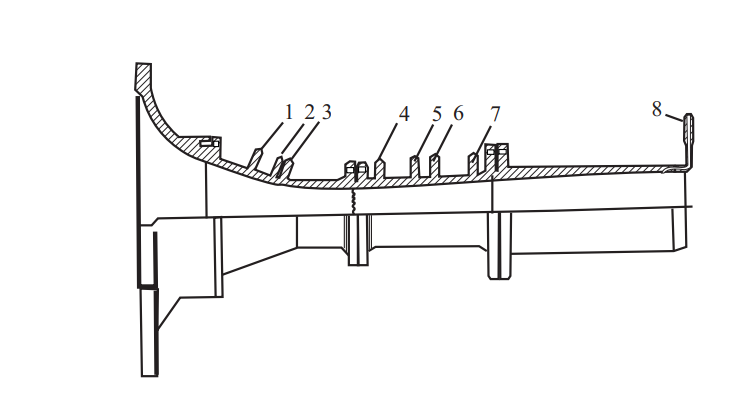
\includegraphics[width=0.85\textwidth]{photos/truba.PNG}
    \caption{Схема сопла Лаваля с дренажными сечениями 1--8}
    \label{fig:truba}
\end{figure}

В работе использовалось сопло, рассчитанное на $M \approx 2$.
Диаметр выходного сечения $d_{\text{вых}} = 110$~мм; критическое
сечение~--- дренаж №\,4 ($2r_* = 82{,}7$~мм). Геометрия дренажных
сечений приведена в табл.~\ref{tab:geom}.

\begin{table}[H]
    \centering
    \caption{Геометрия дренажных сечений сопла ($x$~--- от входа в сопло)}
    \label{tab:geom}
    \begin{tabular}{cccc}
        \toprule
        № дренажа & $x$, мм & $2r$, мм & Примечание \\
        \midrule
        1 & 166{,}5 & 119{,}6 &  \\
        2 & 200{,}5 & 94{,}4  &  \\
        3 & 217{,}5 & 88{,}5  &  \\
        4 & 365{,}5 & 82{,}7  & критическое сечение \\
        5 & 424{,}5 & 83{,}9  &  \\
        6 & 451{,}5 & 85{,}5  &  \\
        7 & 511{,}5 & 92{,}4  &  \\
        8 & 832{,}5 & 110{,}0 & рабочее (выходное) сечение \\
        \bottomrule
    \end{tabular}
\end{table}

% ---------------------------------------------------------------
\section{Результаты и обсуждение}
% ---------------------------------------------------------------

\subsection{Параметры атмосферы и установки}

\begin{table}[H]
    \centering
    \caption{Условия эксперимента}
    \label{tab:atm}
    \begin{tabular}{ll}
        \toprule
        Параметр & Значение \\
        \midrule
        Атмосферное давление $p_0 = p_{\text{атм}}$
            & $742$~мм~рт.~ст.\ $= 98{,}92$~кПа \\
        Температура сухого термометра $T_{\text{сух}}$
            & $24{,}1^\circ$C \\
        Температура смоченного термометра $T_{\text{см}}$
            & $19{,}0^\circ$C \\
        Относительная влажность $r_0$ (по психрометрической таблице)
            & $0{,}60$ \\
        Температура торможения $T_0$
            & $297{,}25$~К \\
        Объём газгольдеров $V$
            & $240$~м$^3$ \\
        Давление в ёмкостях в начале пуска $p_e$
            & $2464$~Па \\
        Давление в ёмкостях при срыве режима $p_{e\,\min}$
            & $23{,}69$~кПа \\
        Время работы (эксперимент) $t_{\mathrm{work}}^{\mathrm{exp}}$
            & $60{,}0$~с \\
        \bottomrule
    \end{tabular}
\end{table}

\subsection{Распределение статического давления вдоль сопла}

По геометрии табл.~\ref{tab:geom} вычислялось $q = F_*/F_i$; затем по
изоэнтропическим соотношениям~--- теоретические $M_{\mathrm{th}}$ и
$p_{\mathrm{th}} = p_0\,\pi(M)$.

\begin{table}[H]
    \centering
    \caption{Статическое давление вдоль сопла: эксперимент и одномерная теория}
    \label{tab:pst}
    \begin{tabular}{c c c c c c}
        \toprule
        № & $F_*/F$ & $M_{\mathrm{th}}$ & $p_{\mathrm{th}}$, кПа
          & $p_{\mathrm{exp}}$, кПа & $p_{\mathrm{exp}}/p_0$ \\
        \midrule
        1 & 0{,}478 & 0{,}291 & 93{,}27 & 94{,}48 & 0{,}955 \\
        2 & 0{,}768 & 0{,}519 & 82{,}29 & 84{,}99 & 0{,}859 \\
        3 & 0{,}873 & 0{,}639 & 75{,}12 & 76{,}28 & 0{,}771 \\
        4 & 1{,}000 & 0{,}972 & 53{,}94 & 53{,}68 & 0{,}543 \\
        5 & 0{,}972 & 1{,}197 & 40{,}87 & 48{,}29 & 0{,}488 \\
        6 & 0{,}936 & 1{,}306 & 35{,}35 & 42{,}48 & 0{,}429 \\
        7 & 0{,}801 & 1{,}597 & 23{,}33 & 28{,}71 & 0{,}290 \\
        8 & 0{,}565 & 2{,}056 & 11{,}56 & 15{,}44 & 0{,}156 \\
        \bottomrule
    \end{tabular}
\end{table}

\begin{figure}[H]
    \centering
    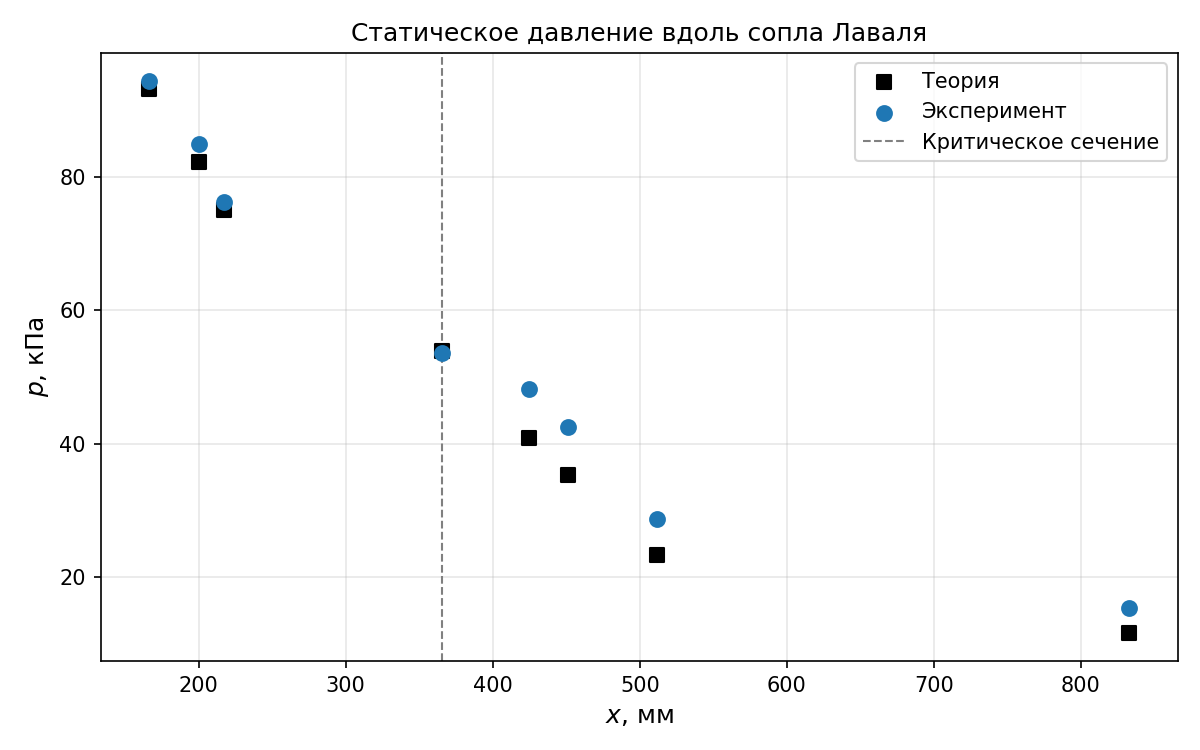
\includegraphics[width=0.92\textwidth]{photos/p_st_x.png}
    \caption{Распределение статического давления вдоль сопла:
             кружки~--- эксперимент, квадраты~--- теория;
             вертикаль~--- критическое сечение.}
    \label{fig:pst}
\end{figure}

Согласие количественно оценим относительной $L^1$-нормой ошибки
\begin{equation}
    \varepsilon_{L^1}
    =
    \frac{1}{N}
    \sum_{i=1}^{N}
    \frac{\bigl|p_{\mathrm{exp},i} - p_{\mathrm{th},i}\bigr|}
         {p_{\mathrm{exp},i}}
    \approx 0{,}103
    \quad (10{,}3\,\%).
    \label{eq:l1}
\end{equation}
В дозвуковой части и в критическом сечении согласие хорошее
(локальные относительные ошибки $\sim 0{,}5$--$3\,\%$); основной вклад в
$\varepsilon_{L^1}$ даёт сверхзвуковая часть, где
$p_{\mathrm{exp}} > p_{\mathrm{th}}$.
Наиболее правдоподобная причина - пограничный слой. 
Дополнительно возможны потери полного давления на трение,
конденсация влаги при $r_0 = 0{,}6$ и отклонение течения от одномерности.

\subsection{Неравномерность поля $p'_0$ и $M$ на срезе сопла}

Среднее $M_{\mathrm{av}}$ считалось по насадкам 3--11 (ядро потока);
насадки 1, 2 и 12 при усреднении не использовались.

\begin{table}[H]
    \centering
    \caption{Полное давление за скачком и $\Delta M$ на срезе сопла}
    \label{tab:pitot}
    \begin{tabular}{c c c c}
        \toprule
        № насадка & $p'_0$, Па & $\Delta M_i = M_i - M_{\mathrm{av}}$ & Примечание \\
        \midrule
        1  & 15762 & $+1{,}013$ & вне ядра \\
        2  & 69044 & $+0{,}070$ & край ядра \\
        3  & 71868 & $+0{,}009$ &  \\
        4  & 72157 & $+0{,}002$ &  \\
        5  & 72853 & $-0{,}013$ &  \\
        6  & 72611 & $-0{,}007$ &  \\
        7  & 71136 & $+0{,}003$ &  \\
        8  & 72925 & $-0{,}014$ &  \\
        9  & 72233 & $+0{,}001$ &  \\
        10 & 71923 & $+0{,}007$ &  \\
        11 & 71671 & $+0{,}013$ &  \\
        12 & 43688 & $+0{,}670$ & вне ядра \\
        \bottomrule
    \end{tabular}
\end{table}

Среднее по ядру (насадки 3--11):
\[
    M_{\mathrm{av}} \approx 1{,}99.
\]
Максимальное относительное отклонение числа Маха в ядре
\[
    \delta M_{\max}
    =
    \max_i \left|
      \frac{M_i - M_{\mathrm{av}}}{M_{\mathrm{av}}}
    \right|
    \approx 0{,}73\,\%.
\]

\begin{figure}[H]
    \centering
    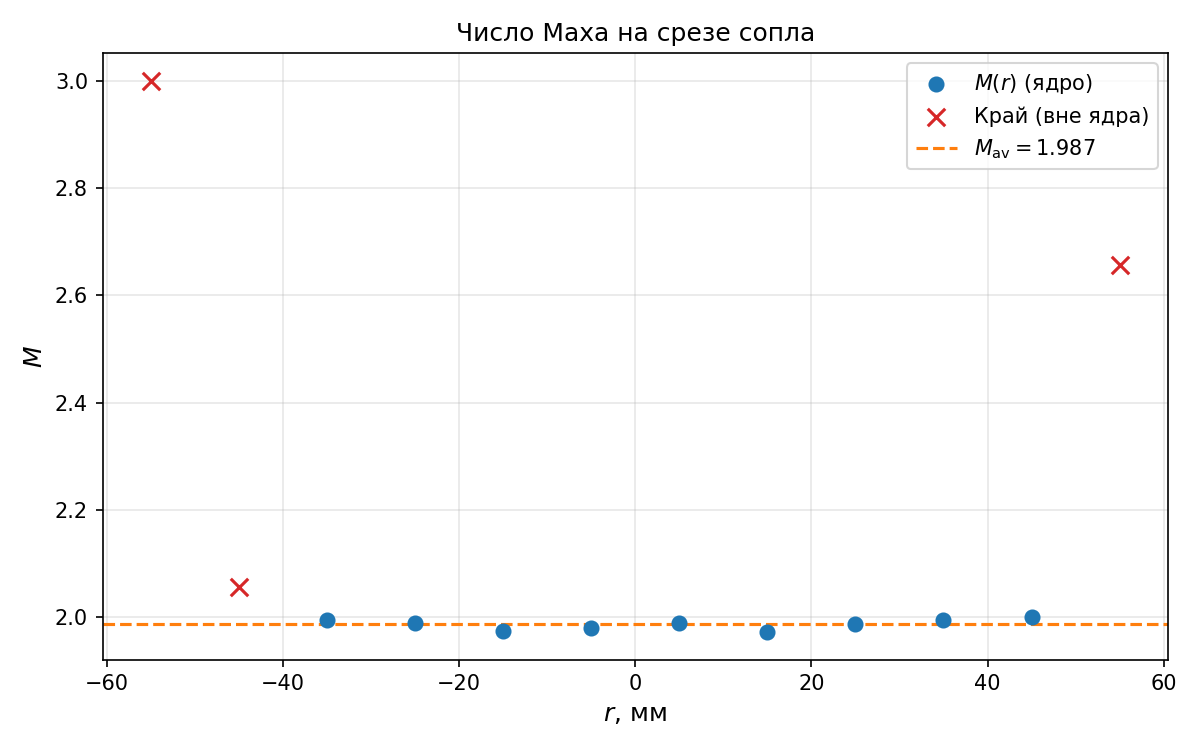
\includegraphics[width=0.92\textwidth]{photos/M_r.png}
    \caption{Профиль числа Маха на срезе сопла. Кружки~--- ядро
             (насадки 3--11), крестики~--- край; пунктир~---
             $M_{\mathrm{av}}$.}
    \label{fig:Mr}
\end{figure}

\begin{figure}[H]
    \centering
    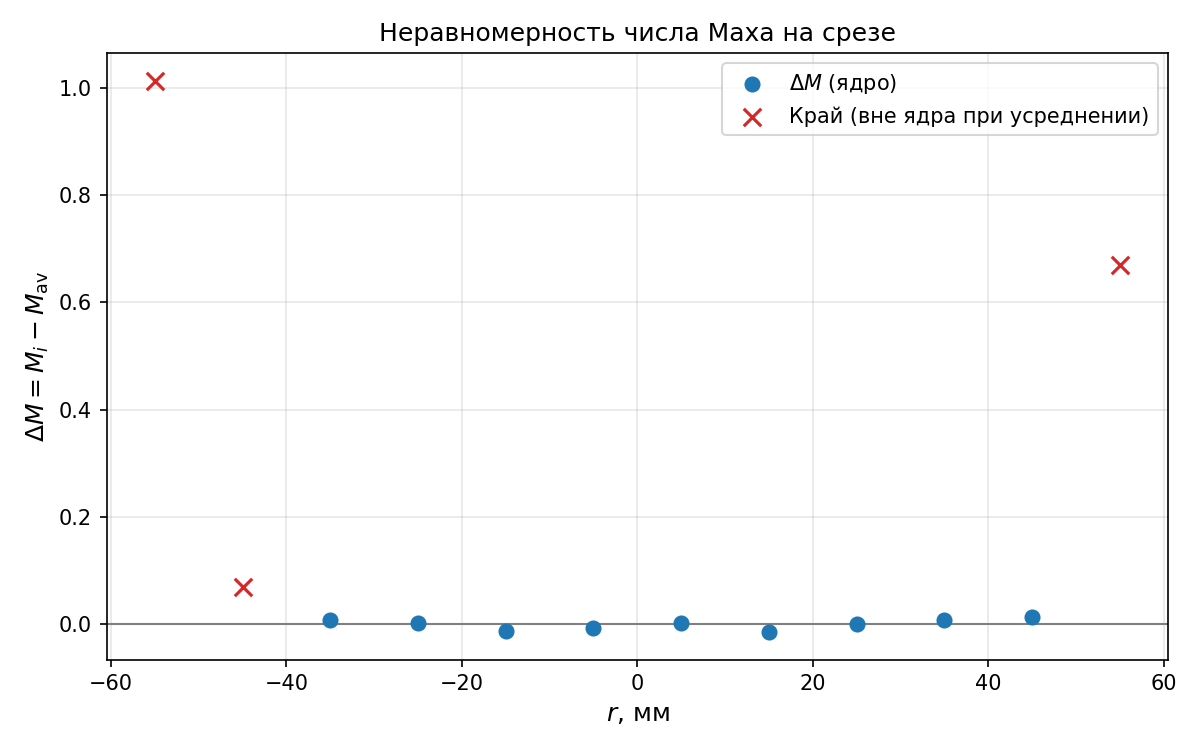
\includegraphics[width=0.92\textwidth]{photos/delta_M_r.png}
    \caption{Неравномерность $\Delta M(r) = M_i(r) - M_{\mathrm{av}}$
             на срезе сопла.}
    \label{fig:dM}
\end{figure}

\begin{figure}[H]
    \centering
    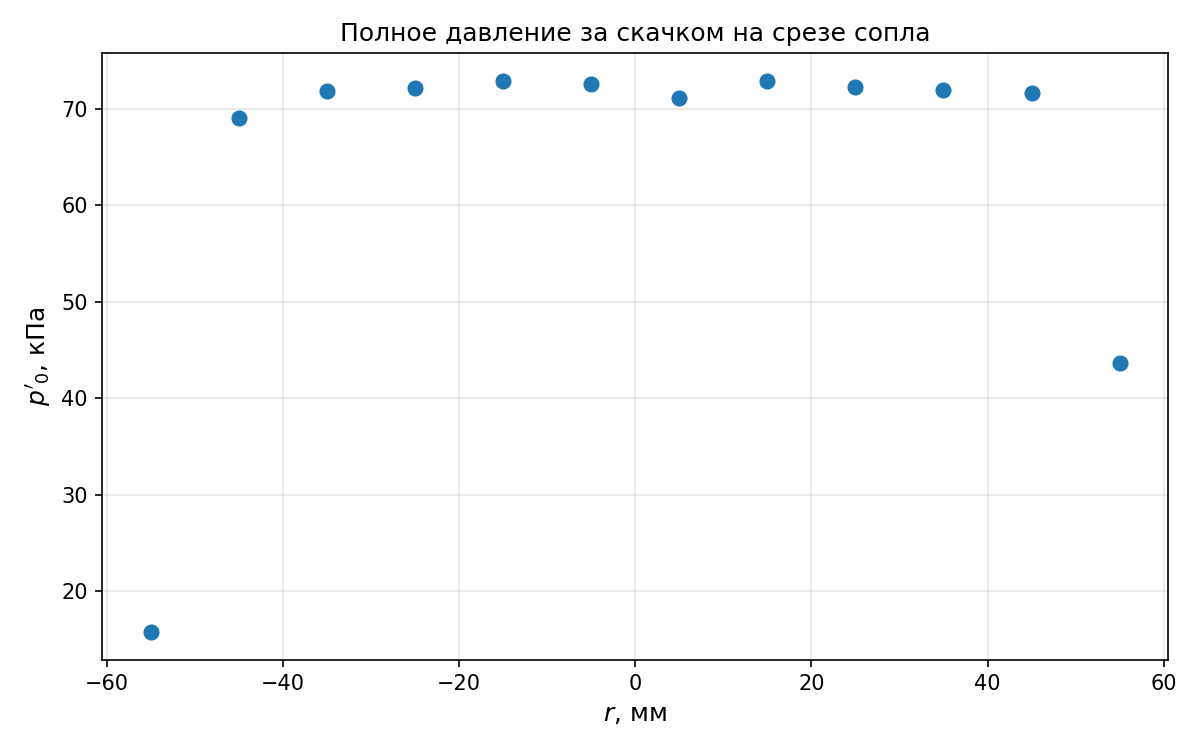
\includegraphics[width=0.92\textwidth]{photos/p0prime_r.png}
    \caption{Полное давление за прямым скачком $p'_0(r)$ на срезе сопла.}
    \label{fig:p0p}
\end{figure}

\subsection{Время работы и степень сжатия}

Площадь критического сечения
$F_* = \pi (d_*/2)^2 = \pi (41{,}35\cdot 10^{-3})^2 \approx 5{,}37\cdot 10^{-3}$~м$^2$.
При $T_0 = 297{,}25$~К, $R = 287$~Дж/(кг$\cdot$К), $\gamma = 1{,}4$:
\[
    a_0 = \sqrt{\gamma R T_0} \approx 346\ \text{м/с},
    \qquad
    \rho_0 = \frac{p_0}{R T_0} \approx 1{,}16\ \text{кг/м}^3,
\]
\[
    Q \approx 1{,}25\ \text{кг/с}.
\]
По формуле~\eqref{eq:twork} при $n = 1{,}1$, $p_e = 2464$~Па,
$p_{e\,\min} = 23{,}69$~кПа:
\[
    t_{\mathrm{work}}^{\mathrm{th}} \approx 46\ \text{с},
\]
тогда как эксперимент дал $t_{\mathrm{work}}^{\mathrm{exp}} = 60$~с.
Расхождение связано с упрощениями модели расхода.

\subsection{Режим истечения}

Статическое давление на срезе сопла $p_c = p_8 = 15{,}44$~кПа.
Давление в газгольдерах в ходе пуска растёт от $p_e$ до $p_{e\,\min}$;
пока $p_{\text{г}} < p_{\text{г max}}$, сверхзвуковой режим в сопле
сохраняется (нерасчётное истечение). По
эмпирической формуле при $M \approx 2$:
\[
    \frac{p_{\text{г max}}}{p_c} \approx 0{,}75\cdot 2 + 0{,}375 = 1{,}875
    \quad\Rightarrow\quad
    p_{\text{г max}} \approx 29\ \text{кПа},
\]
что согласуется по порядку с измеренным $p_{e\,\min} = 23{,}69$~кПа.

\newpage
% ---------------------------------------------------------------
\section{Выводы}
% ---------------------------------------------------------------

\begin{enumerate}
    \item Измерены параметры торможения и влажность:
          $p_0 = 742$~мм~рт.~ст., $T_0 = 24{,}1^\circ$C, $r_0 = 0{,}60$.

    \item Распределение статического давления вдоль сопла систематически
          превышает одномерную теорию.
          В дозвуковой части и в критическом
          сечении согласие хорошее; систематическое превышение
          сосредоточено в сверхзвуковой части.
          Вероятная причина - пограничный слой; вклад могут давать трение, конденсация влаги при $r_0 = 0{,}6$
          и трёхмерность течения.

    \item Среднее число Маха в ядре потока на срезе
          $M_{\mathrm{av}} \approx 1{,}99$ (расчётно $M \approx 2$).
          Неравномерность в ядре: $\delta M_{\max} \approx 0{,}73\,\%$.

    \item Время работы: $t_{\mathrm{work}}^{\mathrm{exp}} = 60$~с,
          расчёт по~\eqref{eq:twork} даёт $\approx 46$~с.
\end{enumerate}

\end{document}
